\section{Theorie}
\label{sec:Theorie}

Treffen Lichtstrahlen auf optisch dichtere oder dünnere Materialen, so werden sie abhängig von der Form  dieser Objekte gebrochen.
Man spricht dabei von Linsen.
Grundsätzlich werden zwei Arten von Linsen unterschieden: Sammellinsen, welche zum Linsenrand dünner werden und das Licht in einem Brennpunkt bündeln, sowie Zerstreuungslinsen, welche eine entgegengesetzte Krümmung besitzen und eine negative Brennweite aufweisen.
Eine Sammellinse erzeugt somit ein reelles Bild, wohingegen eine Zerstreuungslinse ein virtuelles Bild erzeugt.
Die charakteristische Größe eine Linse ist die Brennweite, also die Distanz zwischen der Linse und ihrem Brennpunkt.

\begin{figure}
  \centering
  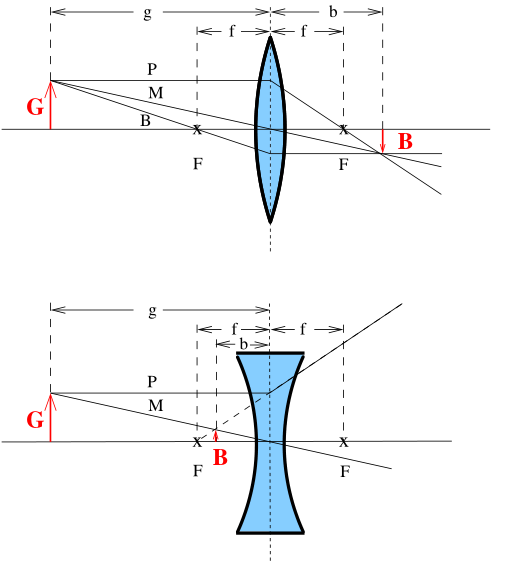
\includegraphics[scale=0.4]{images/Linsen.png}
  \caption{Der Aufbau einer Sammellinse (oben) und einer Zerstreuungslinse (unten), entnommen der Versuchsanleitung \cite[1]{sample}}
  \label{fig:Linsen}
\end{figure}

In Abbildung \ref{fig:Linsen} ist der Aufbau der zwei erwähnten Linsenarten dargestellt.
Die Größe g ist dabei die Gegenstandsweite, also der Abstand zwischen Objekt und Linse,
G ist die Gegenstandsgröße, also die Größe des Objekts,
b ist die Bildweite, also der Abstand zwischen Linse und dem Schirm, bzw. dem Bild,
B ist die Bildgröße, also die Größe des auf dem Schirm sichtbaren Bildes,
und f ist die Brennweite.
Aus den Strahlensätzen und der Bildkonstruktion folgt das Abbildungsgesetz.
Dieses Ist für den Abbildungsmaßstab V wie folgt definiert:

\begin{equation}
  V = \frac{B}{G} = \frac{b}{g}
  \label{eqn:Abbildungsgesetz}
\end{equation}

Für dünne Linsen folgt daraus die Linsengleichung:

\begin{align}
  \frac{1}{f} &= \frac{1}{b} + \frac{1}{g} \\
  f &= \frac{1}{\frac{1}{b} + \frac{1}{g}}
  \label{eqn:Linsengleichung}
\end{align}

Mit ihrer Hilfe kann damit die Brennweite einer Linse berechnet werden

\subsection{Methode nach Bessel}

Bei der Methode anch Bessel wird die Brennweite einer Linse bestimmt, indem man den Abstand zwischen Gegenstand und Bild fest hält und die zwei Linsenpositionen ermittelt, für die das Bild scharf abgebildet wird.
Bei diesen symmetrischen Linsenstellungen sind die Bild- und Gegenstands-weiten vertauschbar:

\begin{align*}
  b_1 = g_2
  \shortintertext{ und }
  b_2 = g_1
\end{align*}

Mit dem Abstand $e = g_1 + b_1 = g_2 + b_2$ zwischen Objekt und Bild , sowie dem Abstand $d = g_1 - b_1 = g_2 - b_2$ zwischen den beiden Linsen ergibt sich für die Brennweite folgende Gleichung:

\begin{equation}
  f = \frac{e^2 - d^2}{4 e}
  \label{eqn:Bessel}
\end{equation}

Der Zusammenhang der Größen ist in Abbildung \ref{fig:Bessel} dargestellt.

\begin{figure}
  \centering
  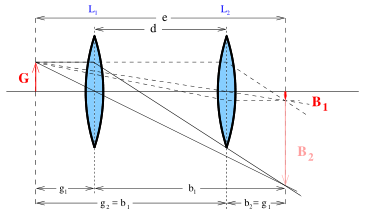
\includegraphics[scale=0.7]{images/Bessel.png}
  \caption{Darstellung der verwendeten Größen, entnommen der Versuchsanleitung \cite[4]{sample}}
  \label{fig:Bessel}
\end{figure}

\subsection{Methode von Abbe}

Bei der Methode von Abbe wird die Brennweite aus dem Abbildungsmaßstab V berechnet.
Hierfür wird ein Linsensystem aus einer Sammel- und einer Zerstreuungs-linse konstruiert.
Dies ist in Abbildung \ref{fig:Abbe} dargestellt.
Da es sich um ein Linsensystem handelt, müssen die Linsen wie dicke Linsen behandelt werden.
Die Größen g und b müssen in Relation zu den Hauptebenen H und H' gemessen werden.
Diese Hauptebenen sind allerdings unbekannt, man muss sich einen beliebigen Punkt A wählen und von dort die Größen g' und b' messen.
Es ergeben sich dann für die Brennweite und die Lage der Hauptebenen folgende Gleichungen:

\begin{align}
  g' &= g + h  = f \cdot \left(1 + \frac{1}{V} \right) + h  \label{eqn:Abbe1}\\
  b' &= b + h' = f \cdot (1 + V) + h'   \label{eqn:Abbe2}
\end{align}

\begin{figure}
  \centering
  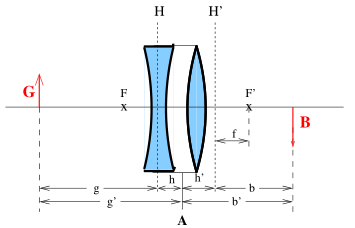
\includegraphics[scale=0.7]{images/Abbe.png}
  \caption{Darstellung des Linsensystems, welches für die Brennweitenbestimmung nach Abbe genutzt wird, entnommen der Versuchsanleitung \cite[5]{sample}}
  \label{fig:Abbe}
\end{figure}
